
\chapter{Egalisation OFDM}

L’égalisation sert à réduire fortement, voir annuler, les interférences dues au
multi-trajets dans le canal de propagation. Dans le domaine temporel, elle se
fait en cherchant les coefficients d’atténuation modélisant l’effet du canal.
Mais, dans le cas de transmission à haut débit, nous avons trop de recouvrement
entre symbole à cause des retards lors de la réception des différents
multi-trajets, ainsi le système devient complexe et donc le coût des terminaux
devient élevé.

L’idée de l’égalisation OFDM est de transformer l’égalisation faite dans le
domaine temporel dans le domaine fréquentiel. En passant dans le domaine
fréquentiel, et en envoyant le signal sur plusieurs porteuses, on est capable
d’évaluer la réponse fréquentielle du canal de propagation sur la bande de
fréquence du signal total. Ce qui est important, c’est que la bande associée à
chaque sous-porteuses doit être dans une zone de cohérence du canal,
c’est-à-dire que la fonction de transfert du canal soit à peu près plat dans la
bande.  Sur l’image ci-dessous, on peut comprendre comment on estime la réponse
fréquentielle du canal par morceaux grâce aux différentes porteuses:

\begin{figure}[!h]
  \centering
  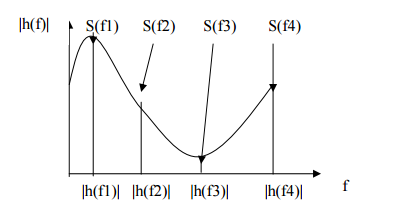
\includegraphics[width=\textwidth]{Porteuses.png}
  \caption{Porteuses}
\end{figure}

Pour égaliser le signal, il suffit de diviser chaque signal reçu par le gain
associé au canal de propagation estimé.

%%% Local Variables:
%%% mode: latex
%%% TeX-master: "../rapport_de_base"
%%% End:
